\documentclass[13pt,dvipsnames,ignorenonframetext,aspectratio = 1610]{beamer}
\setbeamertemplate{caption}[numbered]
\setbeamertemplate{caption label separator}{: }
\setbeamercolor{caption name}{fg=normal text.fg}
\beamertemplatenavigationsymbolsempty
\usepackage{lmodern}
\usepackage{amssymb,amsmath}
% packages
\usepackage{amsfonts, algorithm, algpseudocode, dsfont,
	pgfplots, tikz, tikzscale, ulem, xcolor}
\usetikzlibrary{arrows,shapes,positioning,external}
\pgfplotsset{compat=1.15}

\usepackage{ifxetex,ifluatex}
\usepackage{fixltx2e} % provides \textsubscript
\ifnum 0\ifxetex 1\fi\ifluatex 1\fi=0 % if pdftex
  \usepackage[T1]{fontenc}
  \usepackage[utf8]{inputenc}
\else % if luatex or xelatex
  \ifxetex
    \usepackage{mathspec}
  \else
    \usepackage{fontspec}
  \fi
  \defaultfontfeatures{Ligatures=TeX,Scale=MatchLowercase}
    \setmainfont[]{Roboto Light}
    \setmonofont[Mapping=tex-ansi]{Roboto Mono}
\fi
\usefonttheme{serif} % use mainfont rather than sansfont for slide text
% use upquote if available, for straight quotes in verbatim environments
\IfFileExists{upquote.sty}{\usepackage{upquote}}{}
% use microtype if available
\IfFileExists{microtype.sty}{%
\usepackage{microtype}
\UseMicrotypeSet[protrusion]{basicmath} % disable protrusion for tt fonts
}{}
\newif\ifbibliography
\hypersetup{
            pdftitle={Hierarchical Models and Shrinkage},
            pdfauthor={Jon Fintzi},
            colorlinks=true,
            linkcolor=Maroon,
            citecolor=Blue,
            urlcolor=red,
            breaklinks=true}
%\urlstyle{same}  % Use monospace font for urls

% Prevent slide breaks in the middle of a paragraph:
\widowpenalties 1 10000
\raggedbottom

\AtBeginPart{
  \let\insertpartnumber\relax
  \let\partname\relax
  \frame{\partpage}
}
\AtBeginSection{
  \ifbibliography
  \else
    \let\insertsectionnumber\relax
    \let\sectionname\relax
    \frame{\sectionpage}
  \fi
}
\AtBeginSubsection{
  \let\insertsubsectionnumber\relax
  \let\subsectionname\relax
  \frame{\subsectionpage}
}

\setlength{\parindent}{0pt}
\setlength{\parskip}{6pt plus 2pt minus 1pt}
\setlength{\emergencystretch}{3em}  % prevent overfull lines
\providecommand{\tightlist}{%
  \setlength{\itemsep}{0pt}\setlength{\parskip}{0pt}}
\setcounter{secnumdepth}{0}


\title[Hierarchical Models and Shrinkage]{Hierarchical Models and Shrinkage}
\author[
Jon Fintzi
]{Jon Fintzi}
\institute[
Biostatistics Research Branch
]{
Biostatistics Research Branch \\
National Institute of Allergy and Infectious Diseases\\
National Institutes of Health
}
\date[
09/15/19
]{
September 15, 2019
}

% ------------------------------------------------------------------------------------------------
% BELOW ARE MY ADDITIONS
% ------------------------------------------------------------------------------------------------

% ------------------------------------------------------------------------------------------------
% CUSTOM COMMANDS
% ------------------------------------------------------------------------------------------------
\newcommand{\Var}{\mathrm{Var}}
\newcommand{\E}{\mathrm{E}}
\newcommand{\expit}{\mathrm{expit}}
\newcommand{\logit}{\mathrm{logit}}
\newcommand{\mr}[1]{\mathrm{#1}}
\newcommand{\mb}[1]{\mathbf{#1}}
\newcommand{\mi}[1]{\mathit{#1}}
\newcommand{\bs}[1]{\boldsymbol{#1}}
\newcommand{\rmd}{\mr{d}}
\newcommand{\ind}[1]{\mathds{1}_{\left \lbrace#1\right \rbrace}}
\newcommand{\deriv}[2]{\frac{\rmd#1}{\rmd#2}}
\newcommand{\pdiv}[2]{\frac{\partial#1}{\partial#2}}
\newcommand{\diag}{\mr{diag}}
\newcommand{\wtil}[1]{\widetilde{#1}}
\newcommand{\what}[1]{\widehat{#1}}

\newcommand{\shrug}[1][]{%
	\begin{tikzpicture}[baseline,x=0.8\ht\strutbox,y=0.8\ht\strutbox,line width=0.125ex,#1]
	\def\arm{(-2.5,0.95) to (-2,0.95) (-1.9,1) to (-1.5,0) (-1.35,0) to (-0.8,0)};
	\draw \arm;
	\draw[xscale=-1] \arm;
	\def\headpart{(0.6,0) arc[start angle=-40, end angle=40,x radius=0.6,y radius=0.8]};
	\draw \headpart;
	\draw[xscale=-1] \headpart;
	\def\eye{(-0.075,0.15) .. controls (0.02,0) .. (0.075,-0.15)};
	\draw[shift={(-0.3,0.8)}] \eye;
	\draw[shift={(0,0.85)}] \eye;
	% draw mouth
	\draw (-0.1,0.2) to [out=15,in=-100] (0.4,0.95); 
\end{tikzpicture}}
% ------------------------------------------------------------------------------------------------
%	PACKAGE LIST
% ------------------------------------------------------------------------------------------------
\usepackage{
booktabs,
%fontspec,
graphicx,
multicol,
pgfplots,
ragged2e,
tabularx,
wasysym,
hyperref,
hanging,
multirow,
eso-pic,
}

\usepackage[export]{adjustbox}
% ------------------------------------------------------------------------------------------------
%	GRAPHICS PATH
% ------------------------------------------------------------------------------------------------
\graphicspath{{./figs/}}


% ------------------------------------------------------------------------------------------------
%	TABLE OF CONTENTS
% ------------------------------------------------------------------------------------------------
\useoutertheme[subsection=false,shadow]{miniframes}
\setbeamertemplate{section in toc}[sections numbered]
\setbeamertemplate{subsection in toc}[subsections numbered]

% ------------------------------------------------------------------------------------------------
%	ITEMIZE
% ------------------------------------------------------------------------------------------------
\setbeamertemplate{itemize item}{$\bullet$}
\setbeamertemplate{itemize subitem}{$\circ$}
\setbeamertemplate{itemize subsubitem}{$\bullet$}

\setlength{\parskip}{0.5em}

% ------------------------------------------------------------------------------------------------
%	COLORS
% ------------------------------------------------------------------------------------------------

% sthlm Colors
\definecolor{sthlmLightBlue}{RGB}{0,91,150}
\definecolor{sthlmBlue}{RGB}{3,57,108}
\definecolor{sthlmDarkBlue}{RGB}{1,31,75}
\definecolor{sthlmLightRed}{RGB}{143,39,39}
\definecolor{sthlmRed}{RGB}{124,0,0}
\definecolor{sthlmLightYellow}{RGB}{255,204,0}
\definecolor{sthlmYellow}{RGB}{255,149,0}
\definecolor{sthlmPurple}{RGB}{64,0,64}
\definecolor{sthlmGreen}{RGB}{25,77,51}
\definecolor{sthlmGrey}{RGB}{142,142,147}
\definecolor{sthlmLightGrey}{RGB}{233,233,233}
\definecolor{sthlmDarkGrey}{RGB}{61,61,70}

% General
\setbeamercolor{normal text}{fg=sthlmDarkGrey}
\hypersetup{colorlinks=true, urlcolor=sthlmDarkBlue, linkcolor=sthlmDarkGrey, citecolor=sthlmDarkBlue}
\setbeamercolor{structure}{fg=sthlmDarkGrey}
\setbeamercolor{alerted text}{fg=sthlmRed}
\setbeamercolor{example text}{fg=white}
\setbeamercolor{copyright text}{fg=sthlmLightBlue}
\setbeamercolor{palette primary}{fg=sthlmDarkGrey}
\setbeamercolor{palette secondary}{fg=sthlmDarkGrey,bg=sthlmLightGrey}
\setbeamercolor{palette tertiary}{fg=black,bg=sthlmDarkGrey}
\setbeamercolor{palette quaternary}{fg=white, bg=sthlmDarkGrey}

\setbeamercolor{mini frame}{bg=sthlmLightGrey}
\setbeamercolor{section in head/foot}{fg=sthlmDarkGrey, bg=sthlmLightGrey}

% Titlepage
\setbeamercolor{title}{parent=normal text}
\setbeamercolor{subtitle}{parent=normal text}
\setbeamercolor{institute}{parent=normal text}

% Content
\setbeamercolor{frametitle}{parent=palette quaternary}

% Blocks
\setbeamercolor{block title}{fg=white,bg=sthlmBlue}
\setbeamercolor{block body}{fg=sthlmDarkGrey, bg=sthlmLightGrey}
\setbeamercolor{block title example}{fg=white, bg=sthlmGreen}
\setbeamercolor{block body example}{fg=sthlmDarkGrey, bg=sthlmLightGrey}
\setbeamercolor{block title alerted}{fg=white, bg=sthlmLightRed}
\setbeamercolor{block body alerted}{fg=sthlmDarkGrey, bg=sthlmLightGrey}

% Notes
\setbeamercolor{note page}{fg=sthlmDarkGrey,bg=sthlmLightGrey}
\setbeamercolor{note title}{fg=white, bg=sthlmDarkGrey}
\setbeamercolor{note date}{parent=note title}

% Page Number
\setbeamercolor{page number in head/foot}{fg=sthlmDarkGrey}

\setbeamercolor{qed}{fg=sthlmGrey}
\setbeamercolor{itemize item}{fg=sthlmDarkBlue}
\setbeamercolor{itemize subitem}{fg=sthlmDarkBlue}
\setbeamercolor{itemize subsubitem}{fg=sthlmDarkBlue}

% ------------------------------------------------------------------------------------------------
%	FONTS
% ------------------------------------------------------------------------------------------------

% General

%% Declare fontfamilys
%\if@doNoFlama%
%	% Sans serif math option
%	\if@doSans%
%	% Sans serif math
%		\usepackage{fontspec}%
%		\setmainfont{Arial Regular}%
%	\else%
%		% Serif math
%		\usefonttheme{professionalfonts}%
%		\usepackage[no-math]{fontspec}%
%	\fi%
%	
%	\newfontfamily\Light{Arial Regular}%
%	\newfontfamily\Book{Arial Black Regular}%
%	\newfontfamily\bfseries{Arial Bold}%
%	\setsansfont{Arial Regular}%
%\else%
%	% Sans serif math option
%	\if@doSans%
%	% Sans serif math
%		\usepackage{fontspec}%
%		\setmainfont{FlamaLight}%
%	\else%
%		% Serif math
%		\usefonttheme{professionalfonts}%
%		\usepackage[no-math]{fontspec}%
%	\fi%
%	
%	\newfontfamily\Light{FlamaLight}%
%	\newfontfamily\Book{FlamaBook}%
%	\newfontfamily\bfseries{FlamaMedium}%
%	\setsansfont{FlamaLight}%
%	%\newfontfamily\texttt{SourceCodePro-Light}
%\fi%
%
%%\renewcommand\UrlFont{\texttt}
%
%% Font sizes
%
%% Titlepage
%\setbeamerfont{title}{family=\bfseries,size=\fontsize{24}{26}}
%\setbeamerfont{subtitle}{family=\Light,size=\fontsize{14}{18}}
%\setbeamerfont{subtitle}{size=\fontsize{14}{18}}
%\setbeamerfont{date}{size=\fontsize{9}{11}}
%\setbeamerfont{author}{family=\bfseries,size=\fontsize{13}{15}}
%\setbeamerfont{institute}{size=\fontsize{09}{10}}
%
%% Section
%\setbeamerfont{section title}{size*={39pt}{24pt}, family = \bfseries, series=\bfseries}% Content
%\setbeamerfont{frametitle}{family=\bfseries,size=\large}
%\setbeamerfont{copyright text}{family=\Light,size=\tiny}
%\setbeamerfont{block title}{family=\Book,size=\large}
%\setbeamerfont{block title alerted}{family=\Book,size=\large}
%\setbeamerfont{alerted text}{family=\bfseries}
%
%%Captions
%\setbeamerfont{caption name}{family=\Book}




%% ------------------------------------------------------------------------------------------------
%%	FONT ASSIGMENTS
%% ------------------------------------------------------------------------------------------------
%% Title Page
%\newfontfamily\Light{Roboto Light}
%\setbeamerfont{title}{size=\LARGE, series=\bfseries}
%\setbeamerfont{subtitle}{family=\Light, size=\small, shape=\normalfont}
%\setbeamerfont{date}{family=\Light, size=\footnotesize}
%\setbeamerfont{author}{size=\small, series=\bfseries}
%\setbeamerfont{institute}{family=\Light, size=\scriptsize}
%
%% Section
%\setbeamerfont{section title}{size=\Huge}
%
%% Content
%\setbeamerfont{frametitle}{size=\Large, series=\bfseries}
%\setbeamerfont{copyright text}{size=\tiny}
%\setbeamerfont{block title}{size=\large, series=\bfseries}
%\setbeamerfont{block title alerted}{size=\large, series=\bfseries}
%\setbeamerfont{block title example}{size=\large, series=\bfseries}
%
%\setbeamerfont{caption}{size=\small}
%\setbeamerfont{caption name}{family=\small}

% ------------------------------------------------------------------------------------------------
%	FONT ASSIGMENTS
% ------------------------------------------------------------------------------------------------
% Title Page
%\newfontfamily\Light{Roboto Light}
\setbeamerfont{title}{size=\LARGE, series=\bfseries}
\setbeamerfont{subtitle}{size=\normalsize, shape=\normalfont}
\setbeamerfont{date}{size=\normalsize}
\setbeamerfont{author}{size=\normalsize, series=\bfseries}
\setbeamerfont{institute}{size=\small}

% Section
\setbeamerfont{section title}{size=\Huge}

% Content
\setbeamerfont{frametitle}{size=\Large, series=\bfseries}
\setbeamerfont{copyright text}{size=\tiny}
\setbeamerfont{block title}{size=\large, series=\bfseries}
\setbeamerfont{block title alerted}{size=\large, series=\bfseries}
\setbeamerfont{block title example}{size=\large, series=\bfseries}

\setbeamerfont{caption}{size=\small}
\setbeamerfont{caption name}{family=\small}

% ------------------------------------------------------------------------------------------------
%	TITLE PAGE
% ------------------------------------------------------------------------------------------------

\newcommand\AtPageUpperRight[1]{\AtPageUpperLeft{%
 \put(\LenToUnit{\paperwidth},\LenToUnit{0\paperheight}){#1}%
 }}%
\newcommand\AtPageLowerRight[1]{\AtPageLowerLeft{%
 \put(\LenToUnit{\paperwidth},\LenToUnit{0\paperheight}){#1}%
 }}%

%\AddToShipoutPictureBG*{% Add picture to current page
%  \AtStockLowerLeft{% Add picture to lower-left corner of paper stock
%    \includegraphics[width=\stockwidth,height=\stockheight]{tiger}}% http://latex.tug.org/texlive/devsrc/Master/texmf-dist/doc/generic/pstricks/images/tiger.eps
%}

% Titlepage structure
\def\maketitle{\ifbeamer@inframe\titlepage\else\frame[plain]{\titlepage}\fi}
\def\titlepage{\usebeamertemplate{title page}}
\setbeamertemplate{title page}
%\frame[plain]{\titlepage}
{
	% Add background to title page
  	%\AddToShipoutPictureFG*{\includegraphics[width=\paperwidth]{backgroundiegs.pdf}}
	%\AddToShipoutPictureFG*{
	%	\AtPageLowerRight{\put(-95, 0){
	%		\includegraphics[width=.2\paperwidth]{title_graphic.pdf}}}}
	%\AddToShipoutPictureFG*{\includegraphics[width=\paperwidth]{youngmetro_logo.png}}
	\begin{minipage}[b][\paperheight]{\textwidth}
	%\vspace*{5mm}
	%\includegraphics[height=14mm]{./logo}\par
	\vspace*{20mm}
	\ifx\insertsubtitle\@empty%
	\else%
		{\usebeamerfont{title}\usebeamercolor[fg]{title}\MakeUppercase{\inserttitle}\parskip0pt\par}%
	\fi%
	\ifx\insertsubtitle\@empty%
	\else%
		{\usebeamerfont{subtitle}\usebeamercolor[fg]{subtitle}\insertsubtitle\par}%
		\vspace*{5mm}
	\fi%
	\ifx\insertdate\@empty%
	\else%
		{\usebeamerfont{date}\usebeamercolor[fg]{date}\insertdate\par}%
	\fi% 
	
	\vfill
	
	\ifx\insertauthor\@empty%
	\else%
		{\usebeamerfont{author}\usebeamercolor[fg]{author}\insertauthor\par}%
	\fi%
	\ifx\insertinstitut\@empty%
	\else%
		\vspace*{1mm}
		{\usebeamerfont{institute}\usebeamercolor[sthlmDarkGrey]{institute}\insertinstitute\par}%
	\fi% 
	\vspace*{5mm}
	\end{minipage}
}

% ------------------------------------------------------------------------------------------------
%	SECTION PAGES
% ------------------------------------------------------------------------------------------------

% Make Sectionhead uppercase
\newcommand{\insertsectionHEAD}{%
	\expandafter\insertsectionHEADaux\insertsectionhead}
	\newcommand{\insertsectionHEADaux}[3]{\MakeUppercase{#3}
}

\if@doSectionPage\@empty
\else
% Insert frame with section title at every section start
\AtBeginSection[]
{
\begingroup
\setbeamercolor{background canvas}{bg=sthlmDarkGrey}
\begin{frame}[plain]
\centering
\vfill\usebeamerfont{section title}\textcolor{white}{\insertsectionHEAD}\vfill
\end{frame}
\endgroup
}
\fi

% ------------------------------------------------------------------------------------------------
%	HEADLINE
% ------------------------------------------------------------------------------------------------
\makeatletter
\def\progressbar@progressbar{} % the progress bar
\newcount\progressbar@tmpcounta% auxiliary counter
\newcount\progressbar@tmpcountb% auxiliary counter
\newdimen\progressbar@pbht %progressbar height
\newdimen\progressbar@pbwd %progressbar width
\newdimen\progressbar@tmpdim % auxiliary dimension

\progressbar@pbwd=\paperwidth
\progressbar@pbht=1.25ex

% the progress bar
\def\progressbar@progressbar{%
    \progressbar@tmpcounta=\insertframenumber
    \progressbar@tmpcountb=\inserttotalframenumber
    \progressbar@tmpdim=\progressbar@pbwd
%    \divide\progressbar@tmpdim by 100
%    \multiply\progressbar@tmpdim by \progressbar@tmpcounta
%    \divide\progressbar@tmpdim by \progressbar@tmpcountb
%    \multiply\progressbar@tmpdim by 100
  \begin{tikzpicture}[very thin]

    \shade[top color=sthlmLightGrey,bottom color=sthlmLightGrey,middle color=sthlmLightGrey]
      (0pt, 0pt) rectangle ++ (\progressbar@pbwd, \progressbar@pbht);

      \shade[draw=sthlmDarkBlue,top color=sthlmDarkBlue,bottom color=sthlmDarkBlue,middle color=sthlmDarkBlue] %
        (0pt, 0pt) rectangle ++ (\progressbar@tmpdim, \progressbar@pbht);

  \end{tikzpicture}%
}

\setbeamertemplate{headline}{

  \begin{beamercolorbox}[wd=\paperwidth,ht=1ex,center,dp=0ex]{sthlmLightGrey}%
    \progressbar@progressbar%
  \end{beamercolorbox}%
}

%% ------------------------------------------------------------------------------------------------
%%	FRAME TITLE IN ALL CAPS (MAC: USE "? + ? + }" to uncomment section
%% ------------------------------------------------------------------------------------------------
%\setbeamertemplate{frametitle}
%{
%\begin{beamercolorbox}[wd=\paperwidth,leftskip=0.3cm,rightskip=0.3cm,ht=3ex,dp=1.5ex]{frametitle}
%	 \usebeamerfont{frametitle}\MakeUppercase{\insertframetitle}%
%\end{beamercolorbox}
%}

% ------------------------------------------------------------------------------------------------
%	FRAME TITLE IN TITLE CASE (MAC: USE "? + ? + {" to comment-out section
% ------------------------------------------------------------------------------------------------
\setbeamertemplate{frametitle}
{
\begin{beamercolorbox}[sep=0ex,wd=\paperwidth,leftskip=0.25cm,rightskip=0.3cm,ht=2.75ex,dp=1.375ex]{frametitle}
	 \usebeamerfont*{frametitle}{\insertframetitle}%
\end{beamercolorbox}
}


%\setbeamertemplate{block alerted begin}
%{
%  \setbeamercolor{item}{parent=block body alerted}
%  \par\vskip\medskipamount%
%  \begin{beamercolorbox}[sep=.5ex,dp=0.6ex,leftskip=0.5ex,rightskip=0.5ex]{block title alerted}
%    \usebeamerfont*{block title alerted}\insertblocktitle%
%  \end{beamercolorbox}%
%  {\parskip0pt\par}%
%  {\nointerlineskip\vskip-0.5pt}%
%  \usebeamerfont{block body alerted}%
%  \begin{beamercolorbox}[sep=.5ex,dp=0.6ex,leftskip=0.5ex,rightskip=0.5ex,vmode]{block body alerted}%
%}
%\setbeamertemplate{block alerted end}
%{\end{beamercolorbox}\vskip\smallskipamount}

% ------------------------------------------------------------------------------------------------
%	FOOTLINE
% ------------------------------------------------------------------------------------------------
\usenavigationsymbolstemplate{}
\setbeamertemplate{footline}
{
  \leavevmode%
  \hbox{%
  \begin{beamercolorbox}[sep=0.25ex,wd=.333333\paperwidth,ht=3.25ex,dp=1.25ex,left]{author in head/foot}%
    \usebeamerfont{author in head/foot}\insertshortauthor\expandafter\beamer@ifempty\expandafter{\beamer@shortinstitute}{}{~~--- \insertshortinstitute}
  \end{beamercolorbox}%
  \begin{beamercolorbox}[sep=0.5ex,wd=.333333\paperwidth,ht=3.25ex,dp=1.25ex,center]{title in head/foot}%
    \usebeamerfont{title in head/foot}\insertshorttitle
  \end{beamercolorbox}%
  \begin{beamercolorbox}[sep=0.5ex,wd=.333333\paperwidth,ht=3.25ex,dp=1.25ex,right]{date in head/foot}%
    %\usebeamerfont{date in head/foot}\insertshortdate{}\hspace*{2em}
    Page \insertframenumber{} %/ \inserttotalframenumber\hspace*{2ex} 
  \end{beamercolorbox}}%
  \vskip0pt%
}

% ------------------------------------------------------------------------------------------------
%	CAPTIONS
% ------------------------------------------------------------------------------------------------
\setbeamertemplate{caption label separator}{: }

% ------------------------------------------------------------------------------------------------
%	BLOCKS
% ------------------------------------------------------------------------------------------------
\setbeamertemplate{block begin}
{
  \setbeamercolor{item}{parent=block body}
  \par\vskip\medskipamount%
  \begin{beamercolorbox}[sep=.5ex,dp=0.6ex,leftskip=0.5ex,rightskip=0.5ex]{block title}
    \usebeamerfont*{block title}\insertblocktitle%
  \end{beamercolorbox}%
  {\parskip0pt\par}%
  {\nointerlineskip\vskip-0.5pt}%
  \usebeamerfont{block body}%
  \begin{beamercolorbox}[sep=.5ex,dp=0.6ex,leftskip=0.5ex,rightskip=0.5ex,vmode]{block body}%
}
\setbeamertemplate{block end}  
{\end{beamercolorbox}\vskip\smallskipamount}

\setbeamertemplate{block alerted begin}
{
  \setbeamercolor{item}{parent=block body alerted}
  \par\vskip\medskipamount%
  \begin{beamercolorbox}[sep=.5ex,dp=0.6ex,leftskip=0.5ex,rightskip=0.5ex]{block title alerted}
    \usebeamerfont*{block title alerted}\insertblocktitle%
  \end{beamercolorbox}%
  {\parskip0pt\par}%
  {\nointerlineskip\vskip-0.5pt}%
  \usebeamerfont{block body alerted}%
  \begin{beamercolorbox}[sep=.5ex,dp=0.6ex,leftskip=0.5ex,rightskip=0.5ex,vmode]{block body alerted}%
}
\setbeamertemplate{block alerted end}
{\end{beamercolorbox}\vskip\smallskipamount}

\setbeamertemplate{block example begin}
{
  \par\vskip\medskipamount%
  \begin{beamercolorbox}[sep=.5ex,dp=0.6ex,leftskip=0.5ex,rightskip=0.5ex]{block title example}
    \usebeamerfont*{block title example}\insertblocktitle%
  \end{beamercolorbox}%
  {\parskip0pt\par}%
  {\nointerlineskip\vskip-0.5pt}%
  \usebeamerfont{block body example}%
  \begin{beamercolorbox}[sep=.5ex,dp=0.6ex,leftskip=0.5ex,rightskip=0.5ex,vmode]{block body example}%
}
\setbeamertemplate{block example end}
{\end{beamercolorbox}\vskip\smallskipamount}

% ------------------------------------------------------------------------------------------------
%	BLOCK HOVERING ABOVE THE SLIDE
% ------------------------------------------------------------------------------------------------

\newcommand<>{\hover}[1]{\uncover#2{%
	\begin{tikzpicture}[remember picture,overlay]%
	\draw[fill,opacity=0.4] (current page.south west)
	rectangle (current page.north east);
	\node at (current page.center) {#1};
	\end{tikzpicture}}
	}

% ------------------------------------------------------------------------------------------------
%	VERTICALLY ALIGNED COLUMNS
% ------------------------------------------------------------------------------------------------
	
\usepackage{environ}% Required for \NewEnviron, i.e. to read the whole body of the environment

\newcounter{acolumn}%  Number of current column
\newlength{\acolumnmaxheight}%   Maximum column height


% `column` replacement to measure height
\newenvironment{@acolumn}[1]{%
    \stepcounter{acolumn}%
    \begin{lrbox}{\@tempboxa}%
    \begin{minipage}{#1}%
}{%
    \end{minipage}
    \end{lrbox}
    \@tempdimc=\dimexpr\ht\@tempboxa+\dp\@tempboxa\relax
    % Save height of this column:
    \expandafter\xdef\csname acolumn@height@\roman{acolumn}\endcsname{\the\@tempdimc}%
    % Save maximum height
    \ifdim\@tempdimc>\acolumnmaxheight
        \global\acolumnmaxheight=\@tempdimc
    \fi
}

% `column` wrapper which sets the height beforehand
\newenvironment{@@acolumn}[1]{%
    \stepcounter{acolumn}%
    % The \autoheight macro contains a \vspace macro with the maximum height minus the natural column height
    \edef\autoheight{\noexpand\vspace*{\dimexpr\acolumnmaxheight-\csname acolumn@height@\roman{acolumn}\endcsname\relax}}%
    % Call original `column`:
    \orig@column{#1}%
}{%
    \endorig@column
}

% Save orignal `column` environment away
\let\orig@column\column
\let\endorig@column\endcolumn

% `columns` variant with automatic height adjustment
\NewEnviron{acolumns}[1][]{%
    % Init vars:
    \setcounter{acolumn}{0}%
    \setlength{\acolumnmaxheight}{0pt}%
    \def\autoheight{\vspace*{0pt}}%
    % Set `column` environment to special measuring environment
    \let\column\@acolumn
    \let\endcolumn\end@acolumn
    \BODY% measure heights
    % Reset counter for second processing round
    \setcounter{acolumn}{0}%
    % Set `column` environment to wrapper
    \let\column\@@acolumn
    \let\endcolumn\end@@acolumn
    % Finally process columns now for real
    \begin{columns}[#1]%
        \BODY
    \end{columns}%
}

% ------------------------------------------------------------------------------------------------
%	IMAGES
% ------------------------------------------------------------------------------------------------

\newbox\mytempbox
\newdimen\mytempdimen

\newcommand\includegraphicscopyright[3][]{%
  \leavevmode\vbox{\vskip3pt\raggedright\setbox\mytempbox=\hbox{\includegraphics[#1]{#2}}%
    \mytempdimen=\wd\mytempbox\box\mytempbox\par\vskip1pt%
    \usebeamerfont{copyright text}{\usebeamercolor[fg]{copyright text}{\vbox{\hsize=\mytempdimen#3}}}\vskip3pt%
}}

\begin{document}

% Hide progress bar and footline on titlepage
\begin{frame}[plain]
\titlepage
\end{frame}

\begin{frame}{In conclusion}
\protect\hypertarget{in-conclusion}{}

Every time we have met, we've talked about: \vspace{-0.1in}

\begin{itemize}
\tightlist
\item
  Bayesian inference \emph{always} starts with a model for the
  \textbf{joint distribution} of \(\theta\) and \(y\):.\vspace{-0.1in}
  \[\pi(\theta, y) = f(y|\theta)\pi(\theta) = \pi(\theta|y)m(y).\vspace{-0.1in}\]
\item
  \textbf{Bayes rule} yields the \textbf{posterior distribution}
  \vspace{-0.1in}
  \[\pi(\theta|y) =  \frac{f(y,\theta)}{m(y)} = \frac{f(y|\theta)\pi(\theta)}{m(y)} \propto Likelihood\times Prior.\vspace{-0.1in}\].
\item
  All of the information used in the \emph{update} to our prior is
  encoded in the \textbf{likelihood},\vspace{-0.1in}
  \[L(\mb{y}|\theta) = \prod_{i=1}^N f(y_i|y_{1,\dots,i-1}\theta).\vspace{-0.1in}\]
\end{itemize}

And last time, we talked about:

\begin{itemize}
\tightlist
\item
  Priors for linear regression parameters.
\item
  Workflow, prior and posterior predictive distributions.
\item
  Failure modes of light tailed priors under poorly chosen scales.
\item
  Weakly informative priors as a starting point.
\end{itemize}

\end{frame}

\begin{frame}{Lectures 15-17 of Statistical Rethinking}
\protect\hypertarget{lectures-15-17-of-statistical-rethinking}{}

Multilevel/hierarchical models:

\begin{itemize}
\tightlist
\item
  Account for latent structure:

  \begin{itemize}
  \tightlist
  \item
    Clustering, e.g., students \textless{} classrooms \textless{}
    schools \textless{} districts, meta-analyses.
  \item
    Heterogeneity, lower level units have individual parameters.
  \end{itemize}
\item
  Shrinkage towards population average.
\item
  Improved out of sample performance, don't want to overfit or underfit.
\item
  Some other topics as well: reparameterization, priors on covariances
  for subject level parameters,
\end{itemize}

\end{frame}

\begin{frame}{Plan for today}
\protect\hypertarget{plan-for-today}{}

Shrinkage, hierarchical models, and regularized regression:

\begin{itemize}
\tightlist
\item
  Baseball example\footnote<.->{Borrowing heavily from Carpenter (2018)}
  - batting ability for players in 1970.
\item
  Three different models - complete, partial, and no pooling of
  information.
\item
  Briefly talk about sparse regression with horseshoe priors as another
  example of hierarchical model.
\end{itemize}

\end{frame}

\begin{frame}[fragile]{Take me out to the ballgame}
\protect\hypertarget{take-me-out-to-the-ballgame}{}

Data from the 1970 Major League Baseball season:

\begin{itemize}
\tightlist
\item
  \(N=18\) players.
\item
  Data: \(y_i = Hits_i /AB_i =\) batting average for player \(i\), first
  \(K_i= 45\) at-bats.
\item
  Goal: predict batting average for remainder of the season,
  \(\wtil{y}_i\).
\end{itemize}

\begin{verbatim}
##      Player AB Hits RemainingAB RemainingHits AvgFirst45 AvgRemainder
## 1  Clemente 45   18         367           127  0.4000000    0.3460490
## 2  Robinson 45   17         426           127  0.3777778    0.2981221
## 3    Howard 45   16         521           144  0.3555556    0.2763916
## 4 Johnstone 45   15         275            61  0.3333333    0.2218182
## 5     Berry 45   14         418           114  0.3111111    0.2727273
## 6   Spencer 45   14         466           126  0.3111111    0.2703863
\end{verbatim}

\end{frame}

\begin{frame}{Model 1 - Complete Pooling}
\protect\hypertarget{model-1---complete-pooling}{}

Use a single quantity, \(\rho\), to represent the probability of a hit
for all players.

\begin{itemize}
\tightlist
\item
  Parameter, \(\lambda = \logit(\rho) = \log(\rho/(1-\rho)) =\) log-odds
  of a hit, so the probability of a hit is
  \(\rho = \logit^{-1}(\lambda)= 1/(1+\exp(-\lambda))\).
\item
  Suppose at-bats for each player are independent Bernoulli trials,
  \(y_i \sim Binomial(K_i, \rho) \equiv Binomial(K_i, \logit^{-1}(\lambda))\).
\item
  Complete pooling model, \(\pi(\mb{Y},\lambda)\): \[\begin{aligned}
  \pi(\lambda|\mb{y}) &\propto \pi(\lambda)L(\mb{y}|\bs{\lambda}),\\
  \lambda &\sim N(-1,1), \\
  L(\mb{y}|\lambda) &= \prod_{i=1}^N Binomial(y_i|K_i, \rho).
  \end{aligned}\]
\item
  Note, prior and posterior over \(\lambda\) imply a prior and posterior
  over \(\rho\).
\item
  Prior for \(\lambda\) is weakly informative for \(\rho\); prior median
  (90\% interval) = 0.269 (0.066, 0.656)).
\end{itemize}

\end{frame}

\begin{frame}{Model 1 - Complete Pooling}
\protect\hypertarget{model-1---complete-pooling-1}{}

Fit the model using \texttt{RStanArm} (see Rmarkdown for code).

\begin{itemize}
\tightlist
\item
  Posterior median (90\% Credible interval): 0.26 (0.24, 0.29).
\item
  Posterior distribution of mean batting average (blue histogram) and
  prior (green density):
\end{itemize}

\begin{center}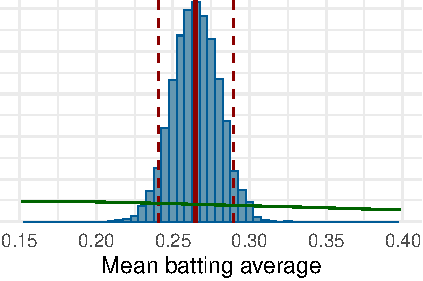
\includegraphics{hierarchical_mods_shrinkage_files/figure-beamer/fit_pool_post-1} \end{center}

\end{frame}

\begin{frame}{Model 2 - No Pooling}
\protect\hypertarget{model-2---no-pooling}{}

Use a different quantity, \(\rho_i\), to independently represent the
probability of a hit for each player.

\begin{itemize}
\tightlist
\item
  Parameter, \(\lambda_i = \logit(\rho_i) = \log(\rho_i/(1-\rho_i)) =\)
  log-odds of a hit for player \(i\), so the probability of a hit is
  \(\rho_i = \logit^{-1}(\lambda_i)= 1/(1+\exp(-\lambda_i))\).
\item
  Suppose at-bats for each player are independent Bernoulli trials,
  \(y_i \sim Binomial(K_i, \rho_i) \equiv Binomial(K_i, \logit^{-1}(\lambda_i))\).
\item
  No-pooling model,
  \(\pi(\mb{Y},\bs{\lambda}) = \pi(\mb{Y}|\bs{\lambda})\prod\pi(\lambda_i)\):
  \[\begin{aligned}
  \pi(\lambda_i|\mb{y}) &\propto \pi(\lambda_i)L(\mb{y}|\bs{\lambda}),\\
  \lambda_i &\sim N(-1,1), \\
  L(\mb{y}|\lambda_i) &= \prod_{i=1}^N Binomial(y_i|K_i, \rho_i).
  \end{aligned}\]
\item
  Note, independent priors and sampling distributions imply independent
  posteriors over \(\lambda_i\).
\end{itemize}

\end{frame}

\begin{frame}{Model 2 - No Pooling}
\protect\hypertarget{model-2---no-pooling-1}{}

\begin{itemize}
\tightlist
\item
  Independent posterior distributions of player-specific batting
  averages are wider.
\item
  Only 45 Bernoulli trials per player, vs.~810 trials with complete
  pooling.
\item
  Posterior distributions of batting averages:
\end{itemize}

\begin{center}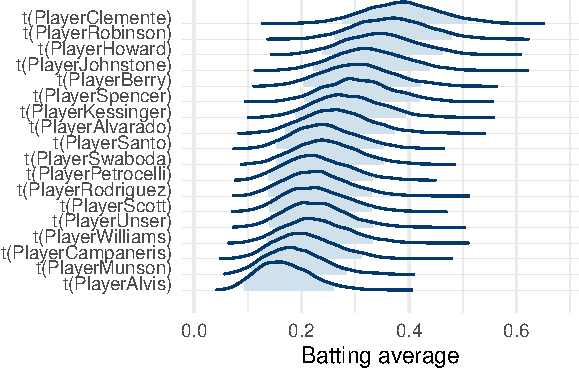
\includegraphics{hierarchical_mods_shrinkage_files/figure-beamer/fit_nopool_posts-1} \end{center}

\end{frame}

\begin{frame}{Model 3 - Partial Pooling}
\protect\hypertarget{model-3---partial-pooling}{}

Use a different quantity, \(\rho_i\), for each player while encoding
that players are similar, not only to themselves, but also to one
another.

\begin{itemize}
\tightlist
\item
  Now, player-level parameters, \(\lambda_i\), have a joint
  distribution, \(\lambda_i \sim \pi(\theta_\lambda)\).
\item
  Partial-pooling model: \[\begin{aligned}
  \pi(\lambda_i|\mb{y}) &\propto \pi(\lambda_i)L(\mb{y}|\bs{\lambda}),\\
  \lambda_i &\sim N(\mu_\lambda, \tau_\lambda^2),\\
  \mu_\lambda &\sim N(-1, 1), \\
  \tau_\lambda &\sim Exponential(1), \\
  L(\mb{y}|\lambda_i) &= \prod_{i=1}^N Binomial(y_i|K_i, \rho_i). \\
  \end{aligned}\]
\item
  Players are no longer independent in this model, rather, they are
  \emph{exchangeable}, a priori.
\item
  Exchangeability
  \(\implies \pi(\lambda_1,\lambda_2) = \pi(\lambda_2,\lambda_1)\), and
  is weaker than independence,
  \(\pi(\lambda_1,\lambda_2) = \pi(\lambda_1)\pi(\lambda_2)\).
\end{itemize}

\end{frame}

\begin{frame}{Model 3 - Partial Pooling}
\protect\hypertarget{model-3---partial-pooling-1}{}

\begin{center}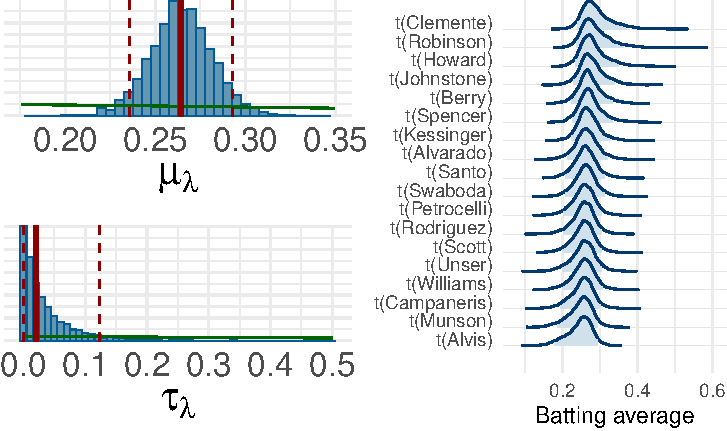
\includegraphics{hierarchical_mods_shrinkage_files/figure-beamer/partialpool_posts-1} \end{center}

\end{frame}

\begin{frame}{Comparing Model Estimates}
\protect\hypertarget{comparing-model-estimates}{}

Partially pooled estimates are a weighted average of the unpooled and
completely pooled estimates, i.e., we are \emph{shrinking} the unpooled
estimates towards the population average hit probability.

\begin{center}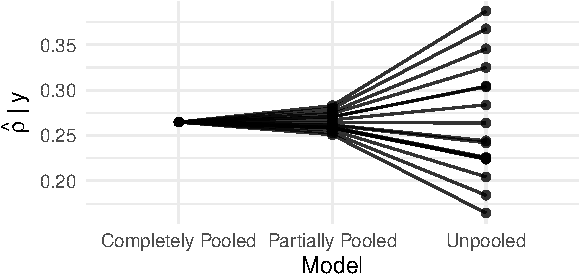
\includegraphics{hierarchical_mods_shrinkage_files/figure-beamer/estcomp-1} \end{center}

\end{frame}

\begin{frame}{Why bother with all this pooling stuff?}
\protect\hypertarget{why-bother-with-all-this-pooling-stuff}{}

A few reasons:\vspace{-0.1in}

\begin{itemize}
\tightlist
\item
  Arguably more faithful to the data generating process.
\item
  Better out of sample predictive performance:

  \begin{itemize}
  \tightlist
  \item
    Expected log predictive density:
    \(elpd_{partial\ pool} = -46.6 \pm 2.2\);
    \(elpd_{no pool} = -53.8 \pm 0.80\).
  \item
    Less uncertainty in prediction intervals:
  \end{itemize}
\end{itemize}

\begin{center}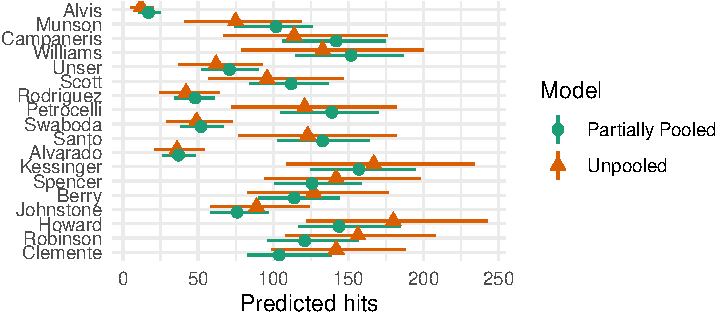
\includegraphics{hierarchical_mods_shrinkage_files/figure-beamer/pp_intervals-1} \end{center}

\end{frame}

\begin{frame}{Summary Before We Continue}
\protect\hypertarget{summary-before-we-continue}{}

Different models for the data and parameters:

\begin{itemize}
\tightlist
\item
  Complete pooling: ignore player labels entirely and lump data.
\item
  No pooling: same as independently analyzing data for each player.
\item
  Partial pooling - players are exchangeable in the prior, estimated
  batting average depends on each player's data and population average.
\end{itemize}

Notice that complete and no pooling are the limiting cases of the
partial pooling model!

\begin{itemize}
\tightlist
\item
  Partial pooling: \(\lambda_i \sim N(\mu_\lambda,\tau_\lambda^2)\)
\item
  Complete pooling, all player-level parameters the same:
  \(\lim_{\tau_\lambda\rightarrow0} N(\mu_\lambda, \tau_\lambda^2)\).
\item
  No pooling, player-level parameters unrelated:
  \(\lim_{\tau_\lambda\rightarrow\infty} N(\mu_\lambda, \tau_\lambda^2)\).
\end{itemize}

\end{frame}

\begin{frame}{The Year is 1998 and Steroids are All the Rage!}
\protect\hypertarget{the-year-is-1998-and-steroids-are-all-the-rage}{}

Fun fact: 1998 was the only year I ever paid attention to baseball.

\begin{itemize}
\tightlist
\item
  Sammy Sosa and Mark Maguire were chasing Roger Maris's home run
  record.
\item
  I was twelve and made my parents get a newspaper subscription so I
  could get updated first thing in the morning.
\item
  Turns out sportsmanship didn't make the majors.
\item
  I became disillusioned. Clearly.
\end{itemize}

\end{frame}

\begin{frame}{The Year is 1998 and Steroids are All the Rage!}
\protect\hypertarget{the-year-is-1998-and-steroids-are-all-the-rage-1}{}

Simulated batting averages over the first 100 at-bats for 250 players
under the following model:\vspace{-0.1in}

\[\begin{aligned}
Y_{i} &\sim Binomial(100, \rho_{i} = \logit^{-1}(\lambda_i)),\ i=1,\dots,250\\
\lambda_i &= \beta_0 + \beta_1X_{roids,i} + \beta_2X_{i,2} + \dots+\beta_{25}0X_{i,25},\ i=1,\dots,250\\
\logit^{-1}(\beta_0) &= 0.269\\
\exp(\beta_1) &= 1.25 \\
X_{roids,i} &= 1,\ i=1,\dots,75; X_{roids,i} = 0,\ i=76,\dots,250,\\
\beta_j &\sim N(0, 0.02^2),\ j=2,\dots,25,\\
X_{i,j} &\sim N(0,1),\ i=1,\dots,250,\ j=1,\dots,25.
\end{aligned}\]

\begin{itemize}
\tightlist
\item
  The thing that matters is steroid use (assumed observed).
\item
  Nothing else matters, and let's suppose we suspect nothing really
  matters.
\end{itemize}

\end{frame}

\begin{frame}{The Year is 1998 and Steroids are All the Rage!}
\protect\hypertarget{the-year-is-1998-and-steroids-are-all-the-rage-2}{}

Simulated data:

\begin{center}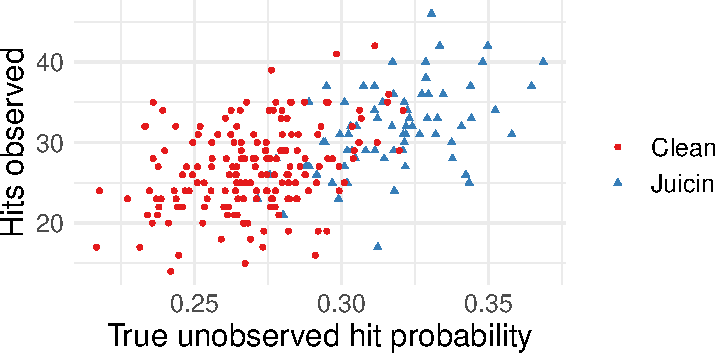
\includegraphics{hierarchical_mods_shrinkage_files/figure-beamer/roid_sim-1} \end{center}

\end{frame}

\begin{frame}{A Simple Hierarchical Model}
\protect\hypertarget{a-simple-hierarchical-model}{}

Partial pooling, as before, but with a bit more complexity b/c of
covariates:

\[\begin{aligned}
Y_{i} &\sim Binomial(100, \rho_{i} = \logit^{-1}(\lambda_i)),\ i=1,\dots,250\\
\lambda_i &= \beta_{talent,i} + \beta_1Z_{roids,i} + \beta_2X_{i,3} + \dots+\beta_250X_{i,25},\ i=1,\dots,250\\
\beta_0 &\sim N(-1,1), \\
\beta_{j} &\sim N(0, 0.42),\ j = 1,\dots,25. 
\end{aligned}\]

\begin{itemize}
\tightlist
\item
  Priors for \(\mu_\lambda\) and \(\tau_\lambda\) are weakly informative
  as before.
\item
  Priors for covariates imply that 90\% of their prior mass of the odds
  ratio of a hit is betwee 0.5x and 2x.
\item
  Note: too many parameters. We know even without fitting this that
  we're looking for trouble.
\end{itemize}

\end{frame}

\begin{frame}{Posterior distributions of model parameters}
\protect\hypertarget{posterior-distributions-of-model-parameters}{}

Posterior distributions of model parameters are overly diffuse.
Uncertainty is sure to propagate into other distributions of interest,
e.g., posterior predictive distributions. \vspace{-0.1in}

\begin{center}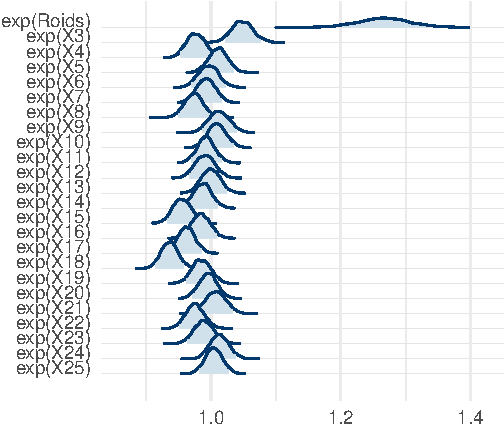
\includegraphics{hierarchical_mods_shrinkage_files/figure-beamer/roid_partial_plot-1} \end{center}

\end{frame}

\begin{frame}{Hierarchical Shrinkage via Horseshoe Priors}
\protect\hypertarget{hierarchical-shrinkage-via-horseshoe-priors}{}

Want to incorporate prior knowledge that many parameters are essentially
zero, but we don't know which ones.

\begin{itemize}
\tightlist
\item
  When \(\beta_i\) is essentially zero, shrink \(\pi(\beta_i|\mb{y})\)
  strongly to zero.
\item
  When \(\beta_i\) is not essentially zero, shrink
  \(\pi(\beta_i|\mb{y})\) very little without leaking posterior mass way
  out into the tails.
\item
  Encode prior information about various aspects of the sparsity, e.g.,
  effective \# of non--zero terms, conditional independence structure,
  etc.

  \begin{itemize}
  \tightlist
  \item
    Computational tractability.
  \end{itemize}
\end{itemize}

This is a tall order!

\end{frame}

\begin{frame}{Hierarchical Shrinkage via Horseshoe Priors}
\protect\hypertarget{hierarchical-shrinkage-via-horseshoe-priors-1}{}

\textbf{Big idea:} prior scale for each model component is a product of
\emph{global} scale and its own \emph{local} scale. \[\begin{aligned}
Y_{i} &\sim Binomial(100, \rho_{i} = \logit^{-1}(\lambda_i)),\ i=1,\dots,250\\
\lambda_i &= \beta_0+ \beta_1Z_{roids,i} + \beta_2X_{i,3} + \dots+\beta_250X_{i,25},\ i=1,\dots,250\\
\beta_0 &\sim N(-1,1), \\
\beta_{j} &\sim N(0, \tau^2\sigma_j^2),\ j = 1,\dots,25,\\
\sigma_j &\sim Cauchy^+(0,1).
\end{aligned}\]

\end{frame}

\begin{frame}{Hierarchical Shrinkage via Horseshoe Priors}
\protect\hypertarget{hierarchical-shrinkage-via-horseshoe-priors-2}{}

\textbf{Intuition:}

\begin{itemize}
\tightlist
\item
  Global scale parameter \(\tau\) shrinks \(\beta_j\) globally to 0.

  \begin{itemize}
  \tightlist
  \item
    Local scales \(\sigma_j\) have Cauchy tails, allowing some
    \(\beta_j\) to escape shrinkage.
  \item
    Varying \(\tau\implies\) more or less sparsity.
  \end{itemize}
\end{itemize}

\textbf{Why horseshoe?}

\begin{itemize}
\tightlist
\item
  Good theoretical properties,
\item
  Good computational properties,

  \begin{itemize}
  \tightlist
  \item
    Not gonna talk about either, see Bhadra (2019).
  \item
    Also
    \href{https://betanalpha.github.io/assets/case_studies/bayes_sparse_regression.html}{\textcolor{blue}{here}}
    for a nice case study.
  \end{itemize}
\end{itemize}

\end{frame}

\begin{frame}{Hierarchical Shrinkage via Horseshoe Priors}
\protect\hypertarget{hierarchical-shrinkage-via-horseshoe-priors-3}{}

Posteriors for irrelevant parameters are strongly shrunk towards zero,
but not the parameter for steroids. Just like we wanted!\vspace{-0.15in}

\begin{center}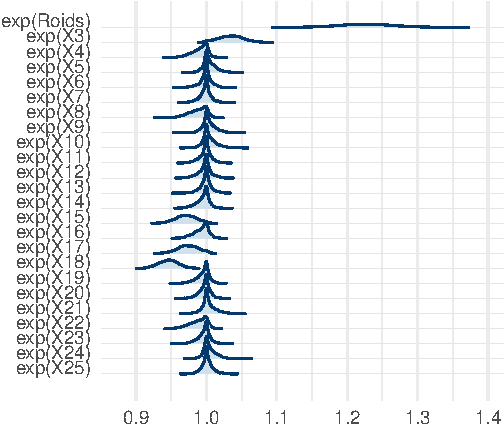
\includegraphics{hierarchical_mods_shrinkage_files/figure-beamer/hs_plot-1} \end{center}

\end{frame}

\begin{frame}{Hierarchical Shrinkage via Horseshoe Priors}
\protect\hypertarget{hierarchical-shrinkage-via-horseshoe-priors-4}{}

Shrinking irrelevant parameters results in better out of sample
predictive performance:

\begin{itemize}
\tightlist
\item
  Expected log predictive density: \(elpd_{HS} - elpd_{partial pool} =\)
  -5.89 \(\pm\) 3.57.
\item
  Less uncertainty in prediction intervals.
\end{itemize}

\end{frame}

\begin{frame}{Summary}
\protect\hypertarget{summary}{}

Iteration on the same idea: construct a joint distribution for data and
parameters.

\begin{itemize}
\tightlist
\item
  Everything starts with a joint distribution.
\item
  We didn't talk about this a lot today, but incredibly important to
  simulate from the prior and interrogate the joint prior distribution.
\item
  Posterior predictive checks for model comparison.
\end{itemize}

Next week is the last lecture. We'll chat about Bayesian handling of
missing data.

\begin{itemize}
\tightlist
\item
  Sneak peak, can think of hierarchical models covered today as a sort
  of missing data problem.
\item
  Lecture 20 of statistical rethinking.
\end{itemize}

\end{frame}

\begin{frame}{References}
\protect\hypertarget{references}{}

A. Bhadra, et al. ``Horseshoe Regularization for Machine Learning in
Complex and Deep Models.'' arXiv preprint arXiv:1904.10939 (2019).

B. Carpenter, et al. ``Hierarchical Partial Pooling for Repeated Binary
Trials.''
\url{https://cran.r-project.org/web/packages/rstanarm/vignettes/pooling.html}
(2018).

B. Efron and C. Morris. ``Data analysis using Stein's estimator and its
generalizations.'' \emph{Journal of the American Statistical
Association} 70.350 (1975): 311-319.

A. Gelman, et al.~Bayesian data analysis. Chapman and Hall/CRC, 2013.

\end{frame}

\begin{frame}{}
\protect\hypertarget{section}{}

\end{frame}

\end{document}